\section{Mehrstufiges, variationales Model}

\begin{figure}[bt]\centering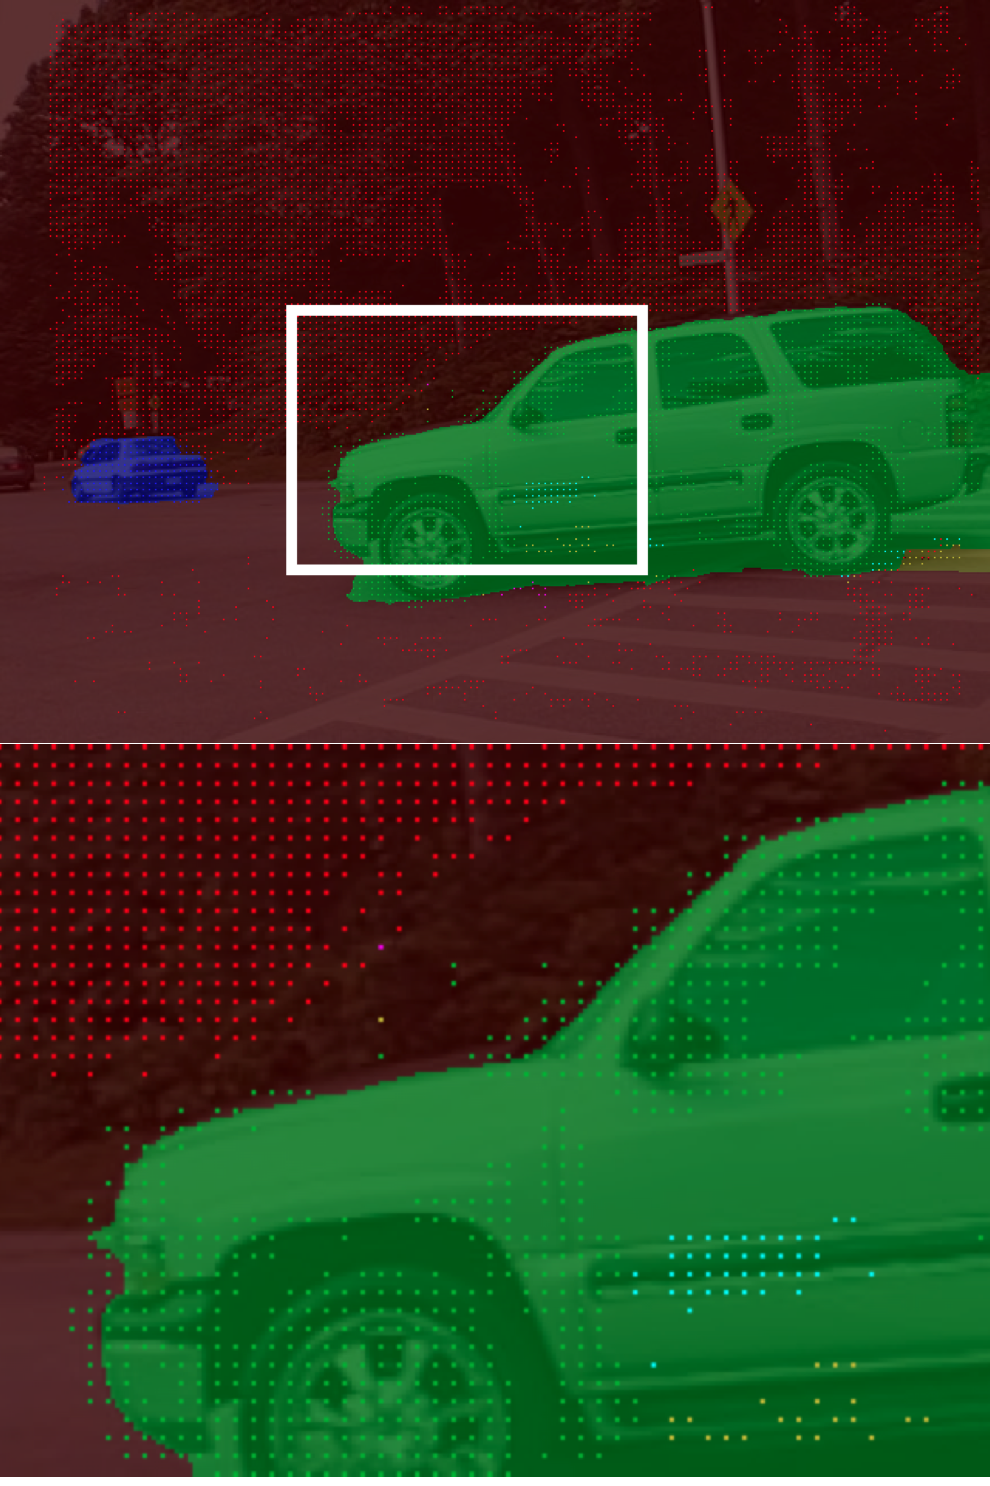
\includegraphics[width=3.5in]{images/close_up_comb.png}
  \caption{Die hellen, einzelnen Punkte sind die Quellpunkte, die durch die Trajektorien erhalten wurden. Die Hintergrundfarbe stellt das endgültige
    Label dar. Oben: Gesamtbild. Unten: Bildausschnitt, zeigt wie selbst die ursprünglich fehlerhaften Quellpunkte korrigiert werden.}
  \label{fig:close}
\end{figure}

\begin{figure}[tb]\centering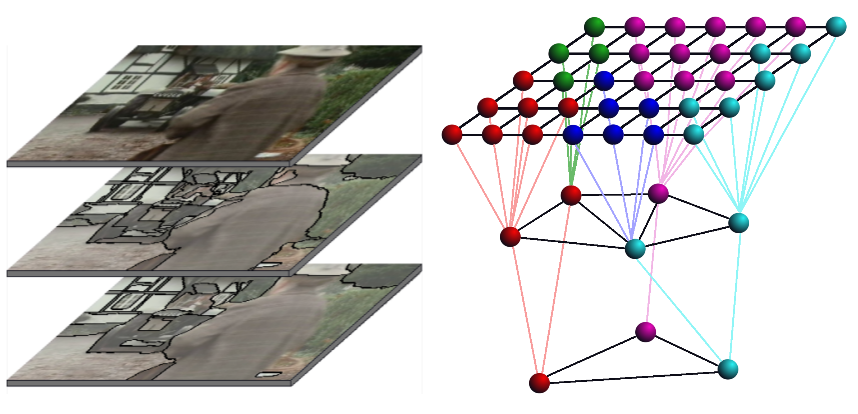
\includegraphics[width=3.5in]{images/graph.png}
  \caption{Stellt die das Schema des mehrstufigen Models da. Links (a): Kontinuierliches Model. Jede Ebene ist eine kontinuierliche Funktion.
  Gröbere Ebenen sind stückweise konstant entsprechend ihrer Superpixel-Unterteilung. Rechts (b): Illustrierung als diskreter Graph}
  \label{fig:graph}
\end{figure}

Die Euler-Lagrange Gleichung aus (\ref{eq:lag1}) kann man auch als nichtlinearen Diffusionsprozess interpretieren.
Dabei dienen die Punkte, die zu einer Trajektorie gehören, als Quellpunkte, um ihre entsprechende Labelinformation zu verbreiten.
Punkte in unmittelbarer Nachbarschaft wirken wie Gegenpole:
Je nachdem wie groß die Labelmasse der Punkte in der Nachbarschaft ist, sowie welcher Wert für $\alpha$ gewählt wurde,
kann ein Quellpunkt $x \in L$ sein Label in der finalen Lösung $u$ auch ändern,
obwohl er immer noch ein Quellpunkt für die dortige, ursprüngliche Labelmasse ist (Abbildung~\ref{fig:close}).

Besonders in homogenen Bereichen ist die Dichte dieser Quellpunkte gering. Dies bedeutet, dass die Information über sehr viel größere Distanzen
propagiert werden muss, meistens behindert durch Rauschen und unwichtige Strukturen. Um dieses Problem zu lösen, soll nun ein mehrstufiges Model zum
Einsatz kommen. Die feinste Ebene dieser Hierarchie entspricht dem zuvor besprochenen, einstufigen Model. Weitere Ebenen nutzen die Information von
Superpixeln, die durch die Anwendung des Verfahrens aus \cite{001} berechnet werden.
Abbildung~\ref{fig:graph}a zeigt eine kontinuierliche Hierarchie, während
Abbildung~\ref{fig:graph}b sie als enstprechende diskrete Graphstruktur zeigt.

Jedes Level $k, k=0,\dotsc,K$ repräsentiert eine kontinuierliche Funktion, die in $M^k$ Superpixel $\Omega_m^k,m=1,\dotsc,M^k$ unterteilt sind.
Für $k=0$ gibt es die Funktionen $u^0$ und $I^0$ wie sie schon im einstufigen Model definiert sind.
Für $k>0$ gibt es die entsprechenden stückweisen konstanten
Funktionen $u^k$ und $I^k$, wobei $I^k(x) = \frac{1}{\Omega_m^k} \int_{\Omega_m^k}I^0(x')dx'$ den mittleren Farbwert aller Punkte des zugehörigen Superpixels
$\Omega_m^k$ annimmt. Die Idee hinter diesen Hilfsfunktionen auf gröberen Ebenen ist es, einen Diffusionsprozess zu definieren, der sich besser der
Bildstruktur auf unterschiedlichen Maßstäben anpasst.

Die Energiefunkion aus (\ref{eq:eng1}) wird nun wie folgt erweitert:
\begin{equation}
\begin{split}
    E(u) &:= \frac{\alpha}{2} \int_\Omega \rho c \sum \limits_{i=1}^n (u_i^0 - \tilde u_i)^2 dx \\
    & + (1-\alpha) \sum \limits_{k=0}^K \int_\Omega g^k \psi \left( \sum \limits_{i=1}^n \left| \nabla u_i^k \right|^2 \right) dx \\
    & + (1-\alpha) \sum \limits_{k=1}^K \int_\Omega g_l^k \psi \left( \sum \limits_{i=1}^n \left| u_i^k -u_i^{k-1} \right|^2 \right) dx,
\end{split}
\label{eq:eng2}
\end{equation}
wobei $u:=(u_1^0,\dotsc,u_n^0,u_1^1,\dotsc,u_n^1,\dotsc,u_1^K,\dotsc,u_n^K)$ nun die Labelfunktion für die gesamte Hierarchie bezeichnet.
Der erste Teil des Terms ist identisch mit dem des einstufigen Models, mit Außnahme der Gewichtungsfunktion $\rho:\Omega \rightarrow \mathbb{R}$,
auf die später noch eingegangen wird. Labelquellen existieren nur auf der feinsten Ebene.
Der dritte Term existiert, um eine Verbindung zwischen den Ebenen herzustellen und genau diese Information von der feinsten Ebene
auf die übrigen zu propagieren. Die Ebenendiffusifitäten $g_l^k$ haben die selbe Bedeutung wie die räumliche Diffusifität $g^k$, nur mit
dem Unterschied, dass sie die Farbwertdistanz zwischen den Ebenen verwenden
\begin{equation}
  g_l^k(x) := \frac{1}{\sqrt{ \left| I^k(x) - I^{k-1}(x) \right|^2 + \varepsilon^2}}, \quad \varepsilon = 0.001
\end{equation}
 im Gegensatz zum Bildgradient $|\nabla I|$.
Der zweite Term in (8) ist die einfache Erweiterung des entsprechenden Terms aus dem einstufigen Model.

Was bringen nun die zusätzlichen Ebenen? Die Superpixel auf den gröberen Ebenen führen zu Bereichen mit konstanten Werten für $I^k$.
Folglich gilt $ \nabla I^k = 0 $ innerhalb eines jeden Superpixels, was wiederum zu einer unendlichen Diffusivität $g^k$ führt.
Mit anderen Worten: Innerhalb eines Superpixels wird die Labelinformation über das gesamte Superpixel mit unendlicher Geschwindigkeit propagiert.
Durch die Verbindung zwischen den Ebenen hat dieser Effekt auch auf die Punkte der nächst feineren Ebene Auswirkungen.
Anstatt den gesamten räumlichen Weg über die feine Ebene, erschwert durch verrauschte Pixel und schwache Strukturen, zurück legen zu müssen,
kann die Information nun eine Abkürzung über die gröberen Ebenen nehmen, wo dieses Rauschen bereits entfernt wurde.

Diese Hierarchie kommt mit dem großen Vorteil einher, dass es nicht notwendig ist, ein richtiges Rauschlevel festzulegen, das unter Umständen
gar nicht global existiert. Stattdessen werden mehrer Ebenen dieser Superpixelhierarchie verwendet und in das Model integriert. Theoretisch
wäre es vorteilhaft, so viele Ebenen wie möglich zu verwenden. Im praktischen Einsatz jedoch empfiehlt es sich, aus Gründen des Berechnungsaufwandes,
diese Anzahl möglichst klein zu halten. Die Authoren empfehlen, das bereits drei Ebenen ausreichen, um bessere Ergebnisse zu erzielen.

Der letzte noch zur Erklärung ausstehende Teil von (\ref{eq:eng2}) ist die Gewichtungsfunktion $\rho$, die es erlaubt ein höheres Gewicht an spezielle Trajektorien
zu verteilen. Der Anreiz dafür liegt darin, dass der verwendete Ansatz von \cite{007} dazu tendiert, falsche Labels an Objektgrenzen auf Grund
von Ungenauigkeiten des optischen Flusses zu liefern. Daher macht es Sinn, den Einfluss von Trajektorien zu erhöhen, die weiter weg von Objektgrenzen liegen,
wohingegen die Labels nahe an den Rändern weniger Einfluss erhalten sollten. Da aber zu diesem Zeitpunkt die Objektgrenzen noch nicht bekannt sind,
werden die Distanzwerte durch Approximation der euklidischen Distanz zu den Superpixelgrenzen $\partial \Omega_m$ auf der gröbsten Ebene angenommen,
welche wiederum sehr effizient berechenbar sind \cite{010}. Basierend auf diesen Distanzen wird
\begin{equation}
\rho(x) := \frac{dist(x, \partial \Omega_m)}{ \frac{1}{|\Omega_m|} \sum_{x\in \Omega_m} dist(x, \partial \Omega_m)}
\end{equation}
definert, mit $x \in \Omega_m$. Dies schließt auch eine Normalisierung der Distanz über die Größe und Form des Superpixels ein.
In großen, homogenen Bereichen, gerade wo der optische Fluss die meisten Probleme hat, erhöht sich $\rho$ langsam mit zunehmender Distanz.
In kleinen Superpixeln, die auf texturstarke Regionen hindeuten, sind selbst Punkte nahen an den Rändern stark gewichtet.

\subsection{Minimierung}

\begin{figure*}[tb]\centering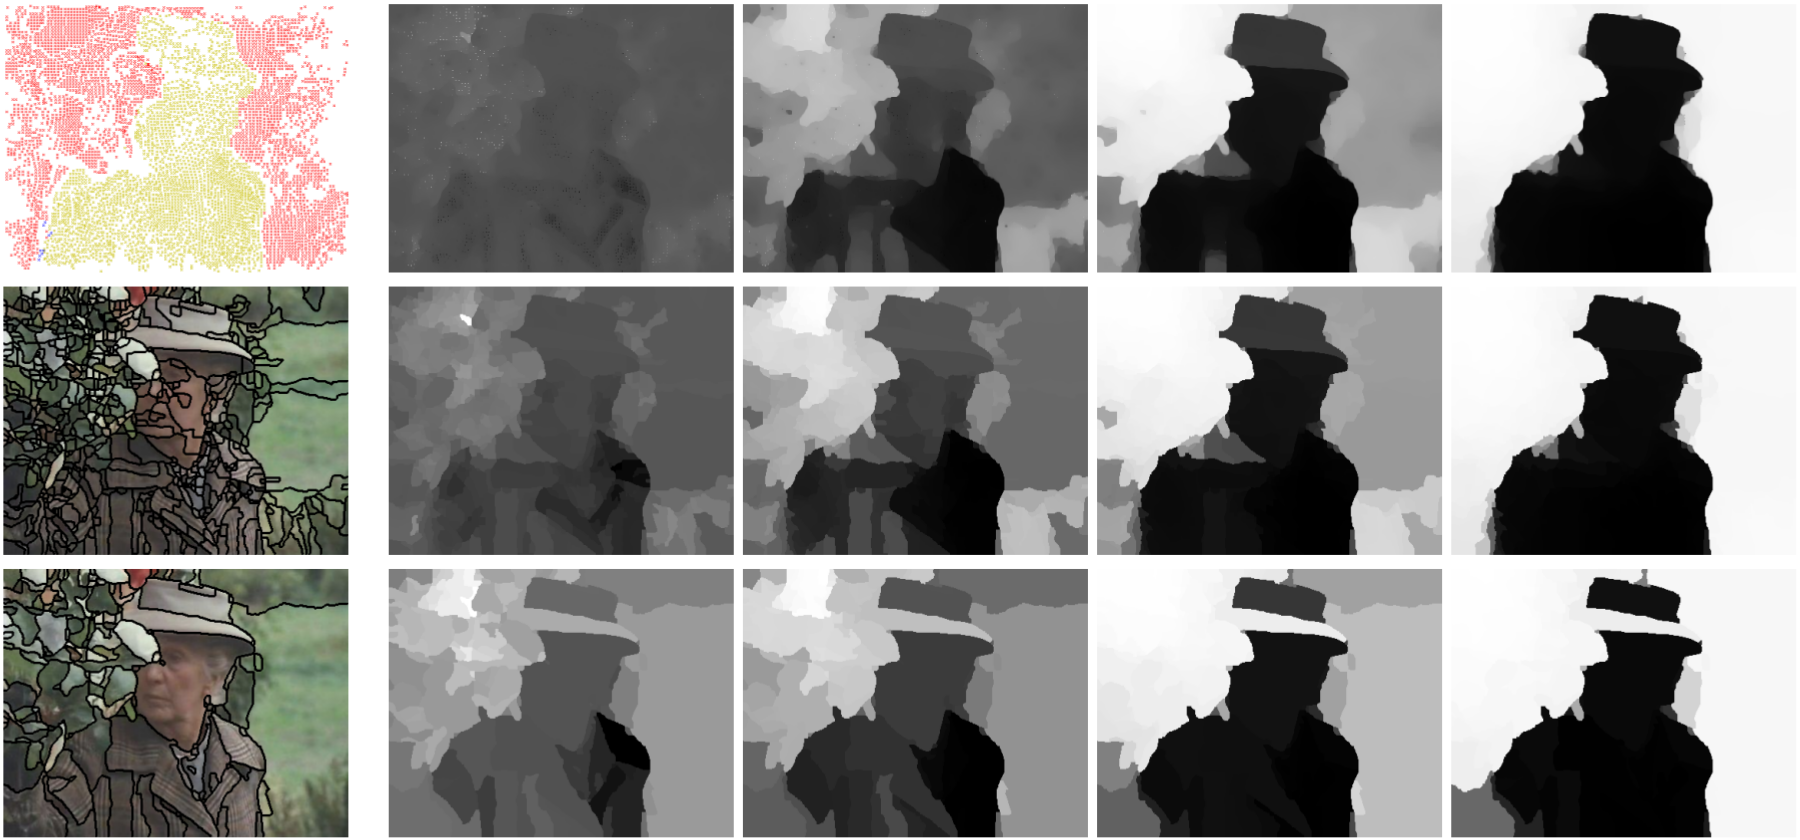
\includegraphics[width=7.0in]{images/evo_labels.png}
  \caption{Links, von oben nach unten: Quellpunkte der Trajektoriencluster, Superpixelbereiche in zwei Stufen.
Rechts: Die Entwicklung der Labelfunktion $u_1^k$ auf allen drei Ebenen gleichzeitig. Zwischenstufen nach 30, 300, 3000 und 30000 Iterationen.}
  \label{fig:evo}
\end{figure*}


Die Minimierung des mehrstufigen Models ist der des einstufigen Models sehr ähnlich.
Die Euler-Lagrange Gleichungen von (\ref{eq:eng2}) für die Ebenen $k>0$ sind
\begin{equation}
\begin{split}
    \mathcal{D}_i^k &:= -\mathrm{div} \left( g^k \psi' \left( \sum \limits_{i=1}^n \left| \nabla u_i^k \right|^2 \right) \nabla u_i^k \right) \\
    & + \left( g_l^k \psi' \left( \sum \limits_{i=1}^n \left| u_i^k - u_i^{k-1} \right|^2 \right) \left| u_i^k - u_i^{k-1} \right|^2 \right)\\
    & - \left( g_l^{k+1} \psi' \left( \sum \limits_{i=1}^n \left| u_i^{k+1} - u_i^{k} \right|^2 \right) \left| u_i^{k+1} - u_i^{k} \right|^2 \right) = 0\\
\end{split}
\end{equation}
für alle $i=1,\dotsc,n$, die ein nichtlineares System mit Variablen auf mehreren Ebenen bilden. Unter Benutzung dieses Terms und den
Neumann-Randbedingungen $u_i^{-1} = u_i^0$ und $u_i^{K+1} = u_i^K$ für alle $i$, ergibt sich daraus die Euler-Lagrange Gleichung für $k=0$
\begin{equation}
    0 = \alpha \rho c (u_i^0 - \tilde u_i) + (1- \alpha) \mathcal{D}_i^0.
\end{equation}
Auch hier lassen sich Fixpunktiterationen zusammen mit SOR anwenden. Abbildung~\ref{fig:evo} zeigt Zwischenschritte dieser iterativen Methode.

%%% Local Variables: 
%%% mode: latex
%%% TeX-master: "../main"
%%% End: 
